\chapter{Implementarea Hardware}
\thispagestyle{pagestyle}

Pentru implementarea hardware am decis să aleg o placă de dezvoltare oferită de Arduino cu performanțe superioare din toate aspectele necesare dezvoltării, și anume Arduino Mega 2560 Rev3. Cu un microcontroler performant aceasta îndeplinește toate criteriile necesare pentru realizarea sistemului. Placa de dezvoltare dispune de 54 de pini digitali, incluzând și toate funcțiile suplimentare de care aveam nevoie: 15 pini ce dispun de PWM, 4 cupluri de pini pentru comunicare serială și pinii pentru comunicarea prin protocolul I2C\cite{mega_datasheet}.

Astfel, cu placa de dezvoltare aleasă și cu arhitectura gândită a început procesul de implementare hardware al componentelor.

\section{Conectarea modulului NodeMCU Lua WIFI ESP8266 CP2102}
Primul pas a fost realizarea comunicării seriale dintre Arduino Mega și modulul NodeMcu pentru a avea acces la WiFi. Modulul trebuie alimentat la 3.3 V fapt ce a fost facilitat de faptul că Arduino Mega dispune de un pin ce oferă o tensiune de 3.3 V fără a mai fi nevoie de un stabilizator de tensiune auxiliar. Apoi, am conectat pinul de GND al plăcii cu cel al modului. Ultimul pas a fost să leg pinii ce realizează comunicarea serială. Am ales a treia interfață serială disponibilă pe Arduino Mega și am conectat pinii dedicați RX (pinul D15) și TX (pinul D14) ai plăcii la pinii dedicați ai modulului RX și TX.
\begin{figure}[H]
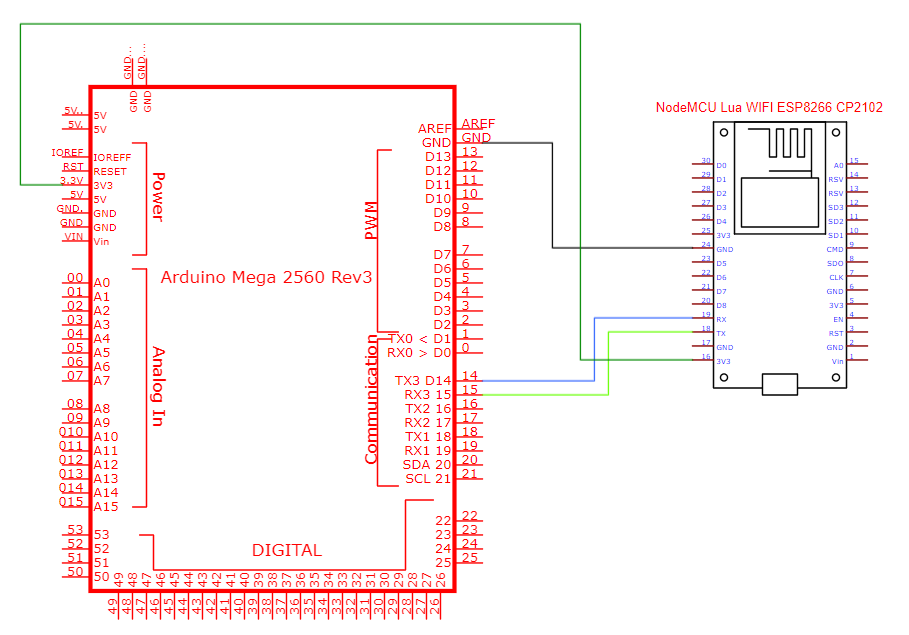
\includegraphics[width=0.9\linewidth]{bachelors_ro/images/conexiune_mega_esp.png}
\caption{Schema de conectare Arduino Mega - NodeMCU}
\label{fig:conexiune_mega_esp}
\end{figure}

\section{Conectarea modulului HC-05}
Următorul pas a fost să realizez comunicarea serială dintre placă și modulul de Bluetooth HC-05. Cele două comunică serial, apoi modulul trimite prin Bluetooth datele mai departe. HC-05 are 6 pini: STATE, RX, TX, GND, 5V, EN. Dintre aceștia a fost nevoie doar de 4. Astfel, pinul de 5V a fost conectat la pinul de alimentare de 5V disponibil pe placa, pinii RX și TX la cuplul RX0 și TX0 al plăcii, iar GND la GND plăcii.

\begin{figure}[H]
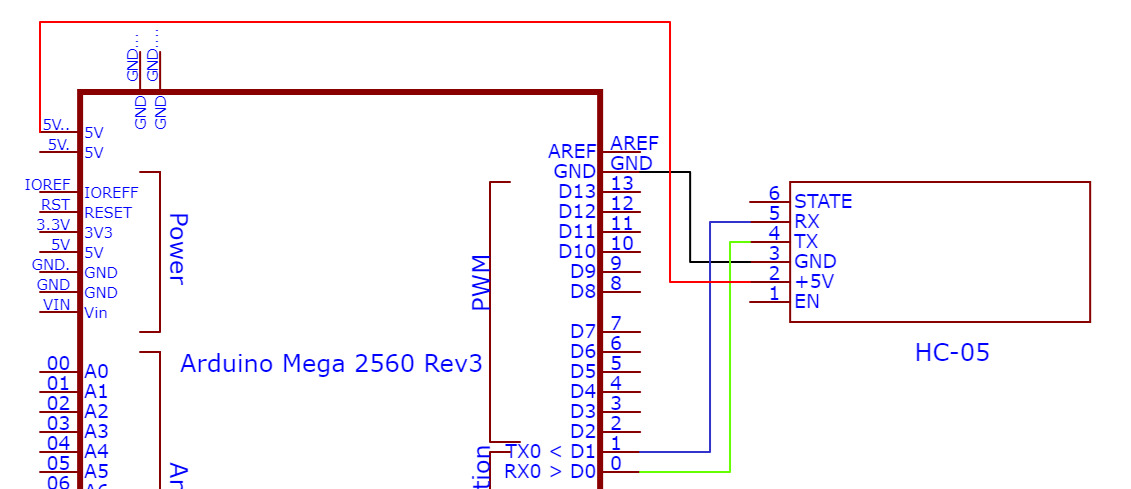
\includegraphics[width=0.7\textwidth, height=0.3\textwidth]{bachelors_ro/images/conexiune_mega_hc05.png}
\caption{Schema de conectare Arduino Mega - HC-05}
\label{fig:conexiune_mega_hc05}
\end{figure}

\section{Conectarea ansamblului de stabilizare a temperaturii}
Montajul ansamblului de stabilizare a temperaturii este format dintr-un senzor de temperatura și umiditate DHT11, un ventilator, un bec H7. Becul și ventilatorul au nevoie de o alimentare de 12 V. Astfel, am ales să folosesc o sursă externă de 12V ce alimentează componentele menționate. Declanșatoarele pentru acestea sunt reprezentate de două relee, ce comută în funcție de o temperatură de prag presetată. În cazul în care temperatura este mai mică decât cea de prag se activează becul, iar dacă este mai mare se activează ventilatorul. 

În Tabelul \ref{tab:conexiune_mega_relee} este prezentată modalitatea în care au fost legați pinii plăcii de cele două relee.
\begin{table}[H]
\caption{Legăturile dintre Arduino Mega și cele doua relee de control}
\label{tab:conexiune_mega_relee}
\begin{tabular}{|l|c|c|c|c|}
\hline
Arduino Mega     & D7 & D11 & 5V & GND \\ \hline
Releu ventilator & S  &     & +  & -   \\ \hline
Releu bec        &    & S   & +  & -   \\ \hline
\end{tabular}
\end{table}

Firul de alimentare de la sursa externă a fost introdus în releu la contactul COM (Common), iar din releu a fost tras un fir de la contactul NC (Normally Closed) la alimentarea ventilatorului. Firul de ground al sursei a fost dus direct la groundul ventilatorului. În aceeași manieră s-a procedat și în cazul becului.
\begin{figure}[H]
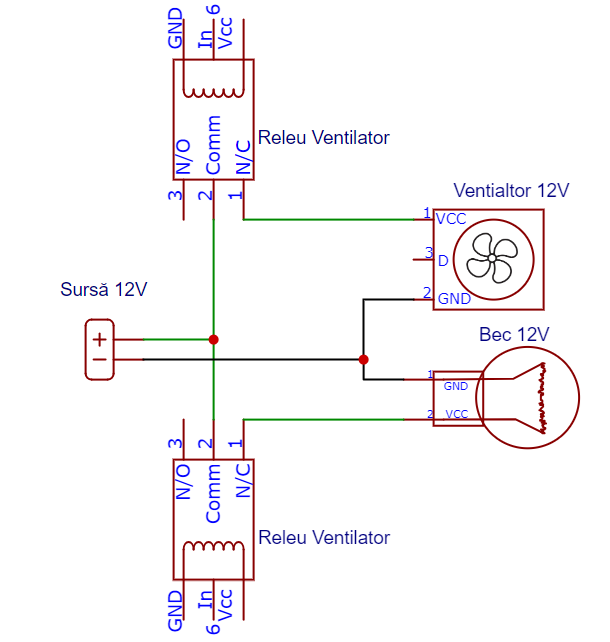
\includegraphics[width=0.6\textwidth, height=0.6\textwidth]{bachelors_ro/images/conexiune_relee_bec_vent.png}
\caption{Schema de conectare Sursă 12V - Relee - Bec/Ventilator}
\label{fig:conexiune_relee_bec_vent}
\end{figure}

Senzorul de umiditate și temperatură DHT11 are 3 pini: S, +, -. Aceștia sunt conectați astfel la placa de dezvoltare.

\begin{table}[H]
\caption{Legăturile dintre Arduino Mega și senzorul DHT11}
\label{tab:conexiune_mega_dht11}
\begin{tabular}{|l|c|c|c|}
\hline
Arduino Mega & D5 & 5V & GND \\ \hline
DHT11 & S & + & - \\ \hline
\end{tabular}
\end{table}

Conform Tabelului \ref{tab:conexiune_mega_relee},\ref{tab:conexiune_mega_dht11} și Figurii \ref{fig:conexiune_relee_bec_vent} ansamblul rezultat este reprezentat în Figura \ref{fig:conexiune_ansamblu_temp}.

\begin{figure}[H]
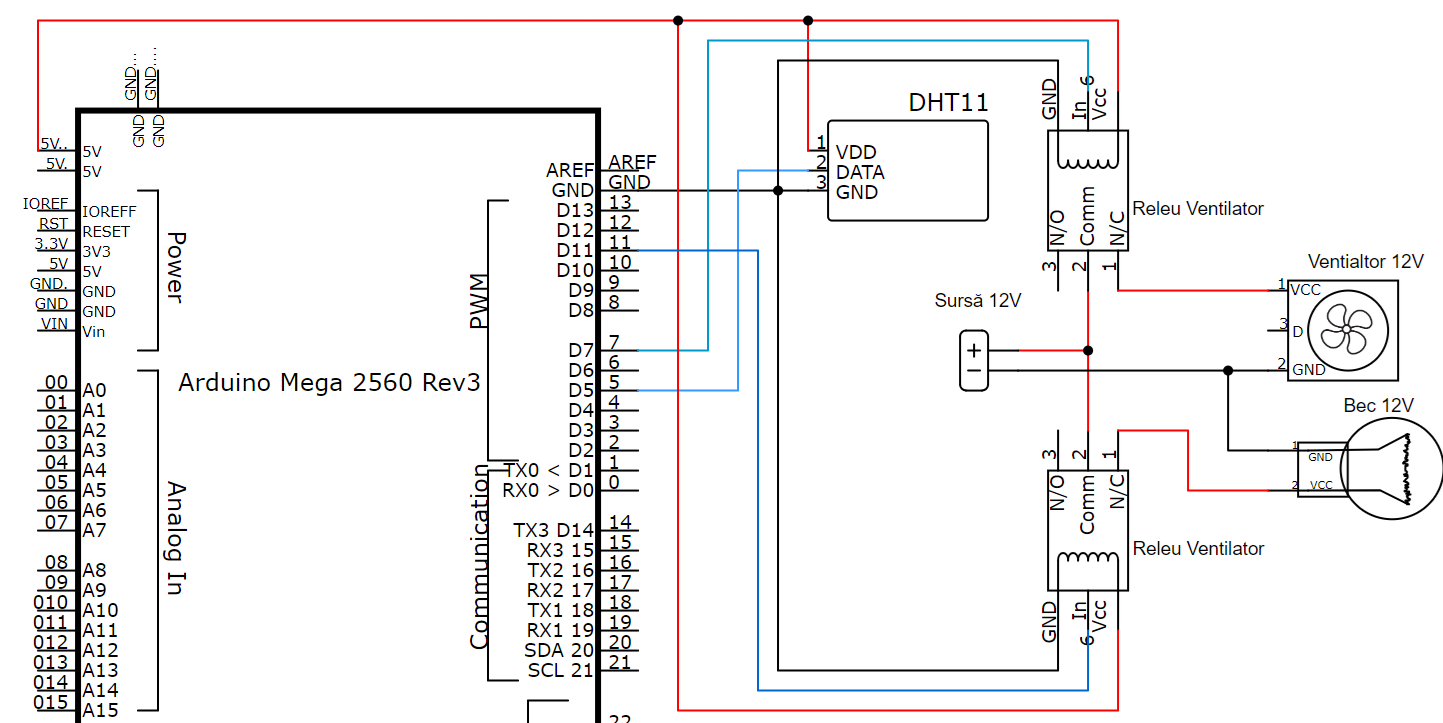
\includegraphics[width=1\linewidth]{bachelors_ro/images/conexiune_ansamblu_temp.png}
\caption{Schema de conectare a ansamblului de stabilizare a temperaturii}
\label{fig:conexiune_ansamblu_temp}
\end{figure}

Ultima componentă pentru a seta temperatura de prag este o tastatură de 4 rânduri și 4 coloane ce permite introducerea acesteia. Tastatura se leagă la 8 pini digitali, 4 pini pentru rânduri și 4 pentru coloane. Legăturile se realizează conform Tabelului \ref{tab:conexiune_tastaura}

\begin{table}[H]
\caption{Legăturile dintre Arduino Mega și Tastatura 4x4}
\label{tab:conexiune_tastaura}
\begin{tabular}{|l|c|c|l|c|l|l|l|l|}
\hline
Arduino Mega & D53 & D51 & D49 & D47 & D45 & D43 & D41 & D39 \\ \hline
Tastatură 4x4 & ROW1 & ROW2 & ROW3 & ROW4 & COL1 & COL2 & COL3 & COL4 \\ \hline
\end{tabular}
\end{table}

Astfel, în Figura \ref{fig:conexiune_tastatura} este prezentat modul de legătură dintre tastatura 4x4 și Arduino Mega.

\begin{figure}[H]
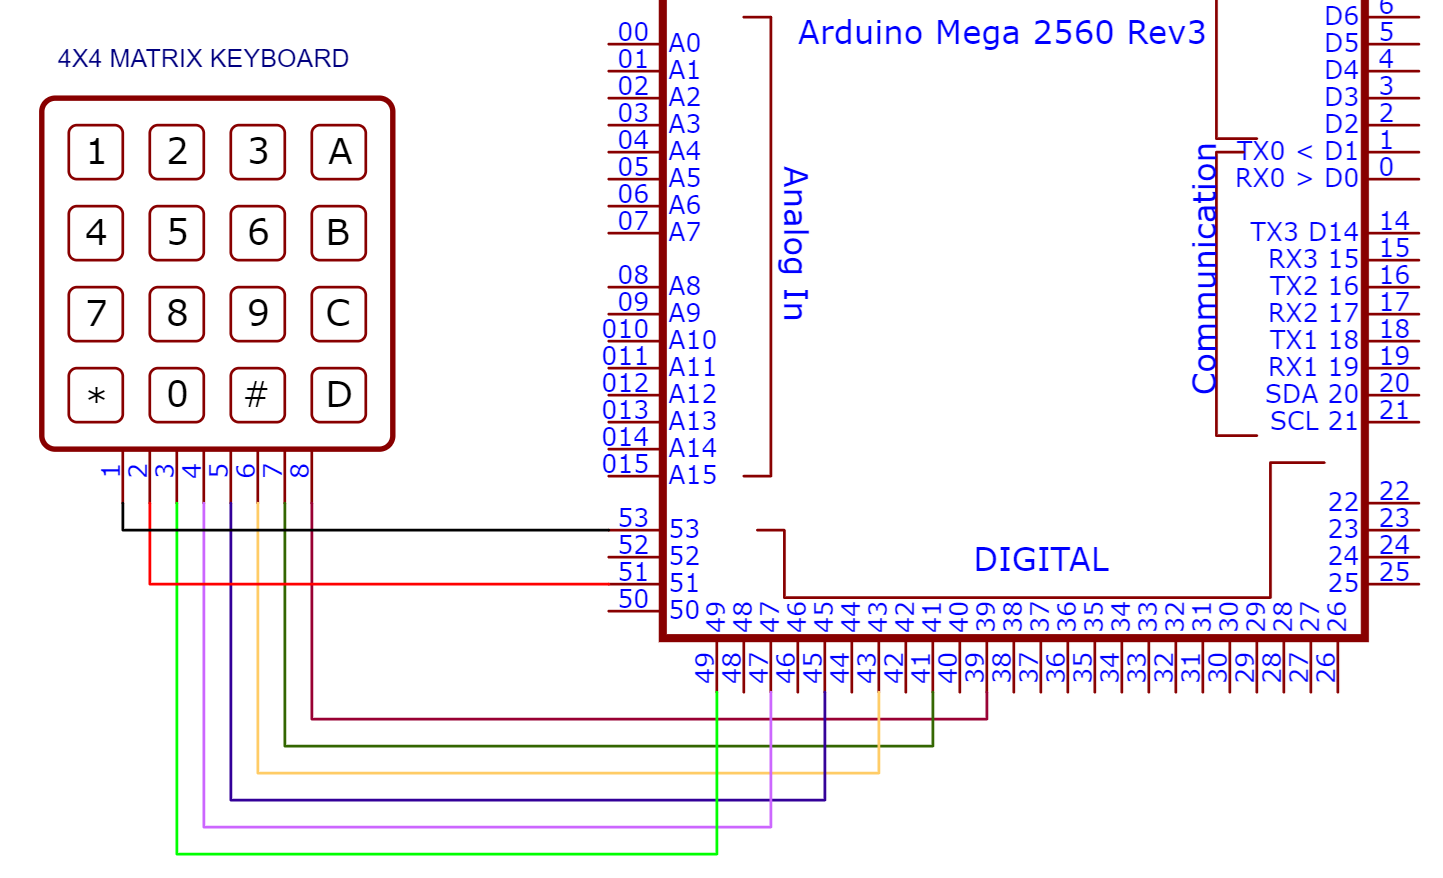
\includegraphics[width=0.5\linewidth]{bachelors_ro/images/conexiune_tastatura.png}
\caption{Schema de conectare dintre tastatură și Arduino Mega}
\label{fig:conexiune_tastatura}
\end{figure}

\section{Conectarea Senzorului de presiune barometrică și a display-ului LCD cu ajutorul protocolului I2C}
Atât senzorul de presiune barometrică BMP280, cât și display-ul LCD 1602 comunică cu placa Arduino Mega prin intermediul protocolului I2C.

În mod tradițional LCD-ul comunică prin mai mulți pini digitali cu placa de dezvoltare, însă celui folosit în proiect i-a fost adăugat o interfață ce permite comunicarea acestuia cu Arduino Mega utilizând protocolul I2C. Astfel, numărul de pini folosiți pentru comunicare a fost redus de la 16 la doar 4 pini specifici modulelor ce folosesc I2C: VCC, GND, SDA (Serial Data Line) și SCL (Serial Clock Line). Echivalent, senzorul de presiune barometrică dispune de exact aceiași pini.

Senzorul de presiune barometrică BMP280 dispune de 6 pini: VCC, GND, SDA, SCL, CSD, SD0. Pentru realizarea montajului s-au folosit doar 4 dintre aceștia (VCC, GND, SCL, SDA). Totodată, senzorul are nevoie de o tensiune de alimentare de 3.3 V spre deosebire de LCD, acesta având nevoie de 5 V. Astfel, firul de alimentare nu poate fi comun pentru cele două.

În Tabelul \ref{tab:conexiune_mega_lcd_bmp} este prezentat modul în care trebuie conectate componentele la Arduino Mega utilizând pinii D20 (SDA) și D21 (SCL) dedicați comunicării I2C.

\begin{table}[H]
\caption{Legăturile dintre Arduino Mega și \\componentele ce comunică prin I2C}
\label{tab:conexiune_mega_lcd_bmp}
\begin{tabular}{|l|c|c|c|l|c|}
\hline
Arduino Mega & D20 & D21 & 5V & 3.3V & GND \\ \hline
LCD 1602 & SDA & SCL & VCC & & GND \\ \hline
BMP280 & SDA & SCL & & VCC & GND \\ \hline
\end{tabular}
\end{table}

Ținând cont de faptul că ambele componente folosesc protocolul I2C pentru a comunica cu microcontroler-ul, fiecare are o adresă unică prezentată în Tabelul \ref{tab:adres_i2c}. Master-ul în acesta caz este reprezentat de microcontroler, iar componentele sunt elementele slave. Pentru a comunica, master-ul inițializează comunicarea folosind o condiție de start, apoi trimite adresa dispozitivului cu care dorește să comunice. Astfel, schimbul de date se face folosind linia SDA (Serial data line) și este sincronizat de SCL (Serial clock line). Pentru încheierea transferului, master-ul generează o condiție de stop. 

\begin{table}[H]
\caption{Adresele componentelor de pe magistrala I2C}
\label{tab:adres_i2c}
\begin{tabular}{|l|c|}
\hline
\textbf{Componenta} & \textbf{Adresa} \\ \hline
BMP280              & 0x76            \\ \hline
LCD 1602            & 0x27            \\ \hline
\end{tabular}
\end{table}

Pentru a realiza conexiunile a fost necesară separarea firelor SDA și SCL în două deoarece se pot folosi doar pinii D20 (SDA) și D21 (SCL) pentru a se realiza comunicarea. Astfel, în Figura \ref{fig:conexiune_bmp_lcd} este prezentată realizarea montajului celor două componente.

\begin{figure}[H]
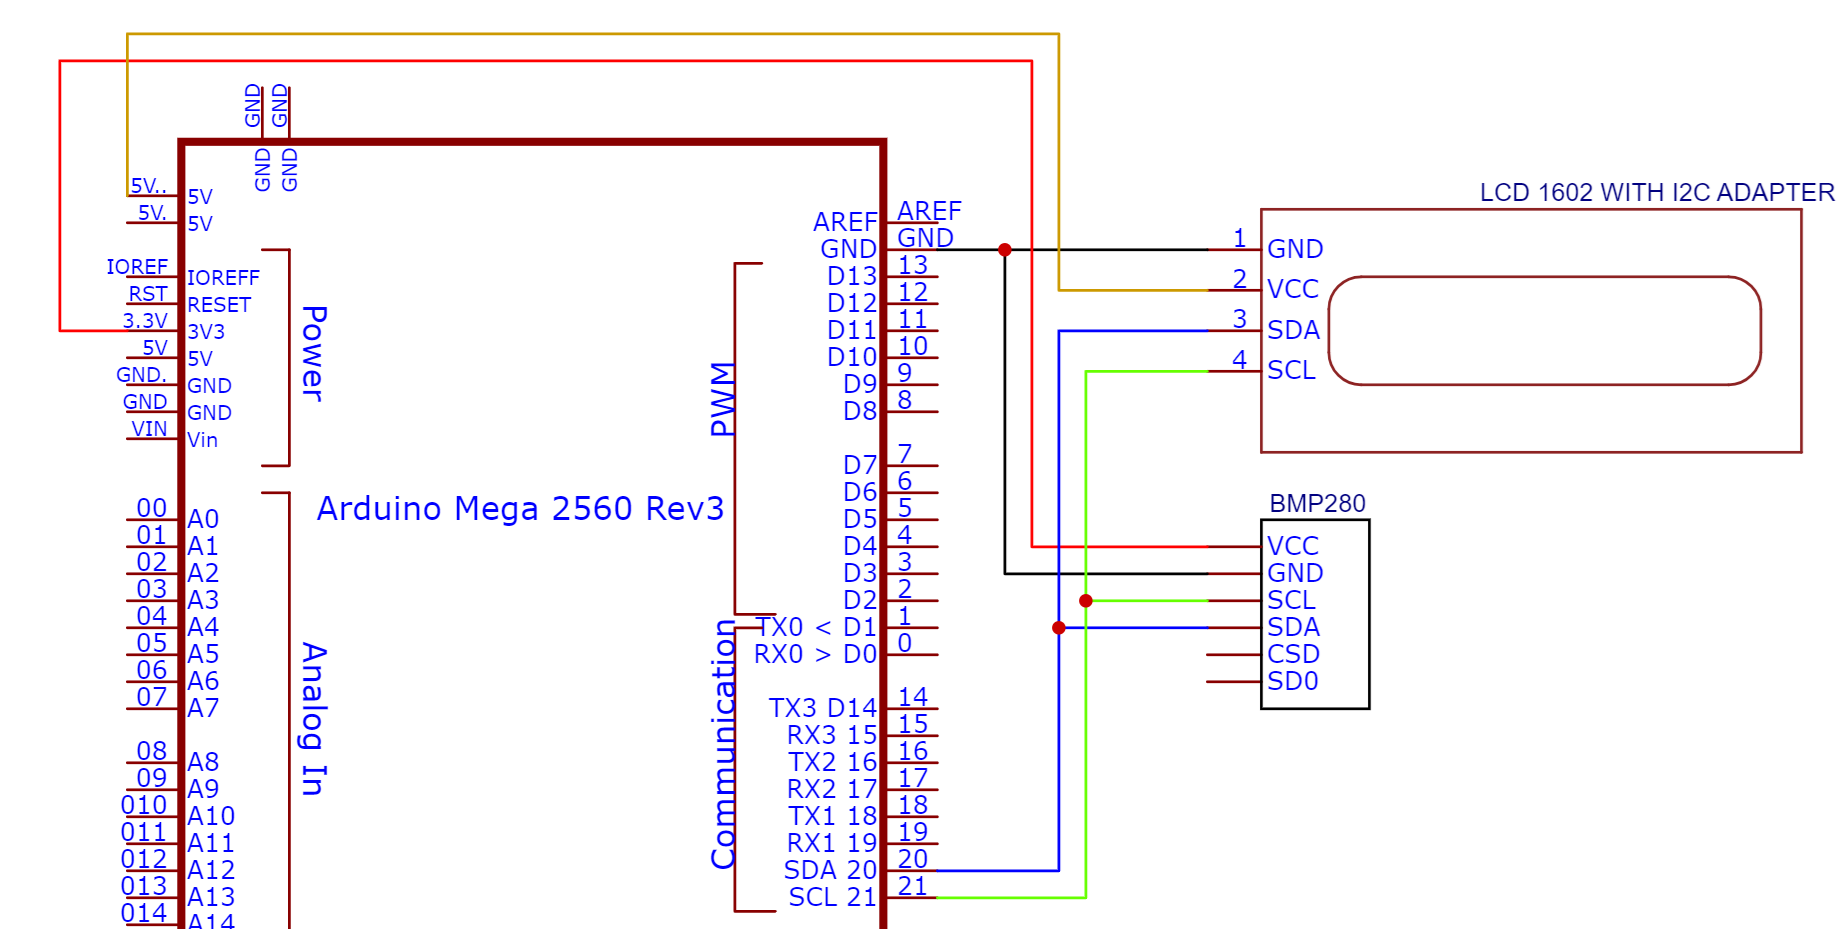
\includegraphics[width=1\textwidth, height=0.5\textwidth]{bachelors_ro/images/conexiune_bmp_lcd.png}
\caption{Schema de conectare a senzorulu de presiune barometrică și a LCD-ului}
\label{fig:conexiune_bmp_lcd}
\end{figure}

\section{Conectarea ansamblului de deschidere automată a ușii}
Ansamblul de deschidere automată a ușii este format din senzorul ultrasonic HC-SR04 și servomotorul SG90. La detectarea mișcării la o anumită distanță predefinită, senzorul trimite un semnal ce activează modificarea poziției servomotorului de la 0 la 180 de grade, astfel deschizând ușa. Apoi, după câteva secunde revine la poziția inițială.

Ambele componente au nevoie de un fir de alimentare comun legat la pinul de 5 V al plăcii și de un GND comun legat la pinul de GND al plăcii. Senzorul ultrasonic trimite date prin pinii ECHO și TRIG către doi pini digitali de pe Arduino Mega, iar servomotorul este controlat folosind un pin digital ce dispune de PWM(Pulse Width Modulation) de pe placă ce este legat la pinul D0 al servomotorului. Astfel, în Tabelul \ref{tab:conexiune_mega_hcsr04_servo} sunt prezentați pinii aleși pentru cele două componente.

\begin{table}[H]
\caption{Legăturile dintre Arduino Mega, Servomotor și Senzorul Ultrasonic}
\label{tab:conexiune_mega_hcsr04_servo}
\begin{tabular}{|l|c|c|c|l|c|}
\hline
Arduino Mega & D9(PWM) & D12 & D13 & 5 V & GND \\ \hline
Servomotor SG90 & D0 & & & VCC & GND \\ \hline
Senzorul HC-SR04 & & TRIG & ECHO & VCC & GND \\ \hline
\end{tabular}

\end{table}

În Figura \ref{fig:conexiune_servo_hcsr04} este prezentat montajul ansamblului format din Arduino Mega, Senzorul Ultrasonic HC-SR04 și servomotorul SG90.

\begin{figure}[H]
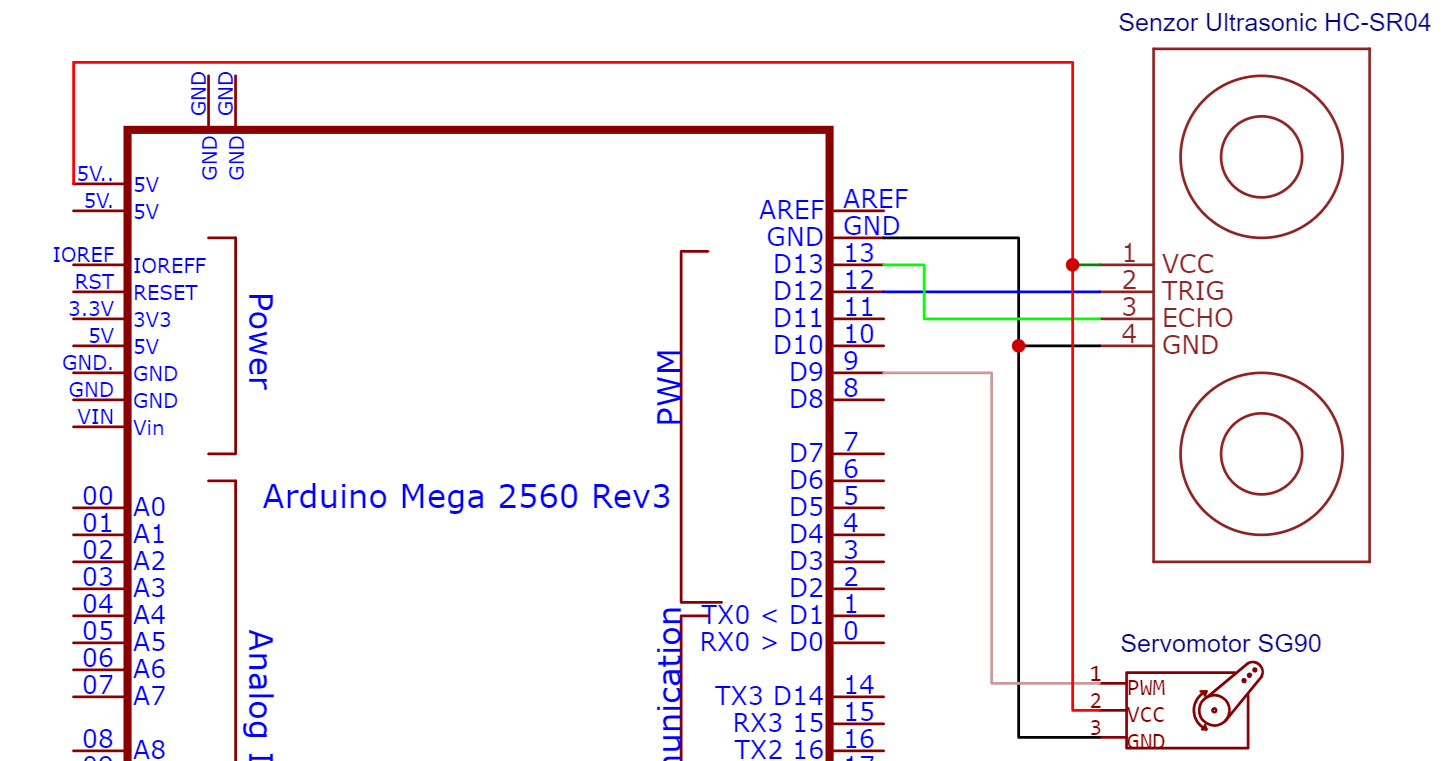
\includegraphics[width=1\textwidth, height=0.6\textwidth]{bachelors_ro/images/conexiune_servo_hcsr04.png}
\caption{Schema de conectare a senzorului ultrasonic și a servomotorului}
\label{fig:conexiune_servo_hcsr04}
\end{figure}

\section{Conectarea ansamblului de alarmă la detectarea gazelor sau a fumului}
Ansamblului de alarmă la detectarea gazelor sau a fumului este format din senzorul MQ2 și un buzzer pasiv. Senzorul este conectat la un pin analogic, acesta oferind date despre concentrația de gaze și fum prezentă în aer. La depășirea unui anumit prag buzzer-ul este activat pentru câteva secunde.

Buzzer-ul este conectat doar la un pin digital împreună cu o rezistență de 100 Ohm și la GND, neavând nevoie de o tensiune de alimentare. Senzorul, în schimb, trebuie conectat și la o tensiune de alimentare de 5 V pe lână pinul analogic și pinul de GND. Totodată, senzorul MQ2 dispune și de un al patrulea pin, DO, ce ar trebui legat la un pin digital pentru a transmite datele înregistrate, dar acest mod este lipsit de acuratețe deci nu va fi folosit. Astfel, în Tabelul \ref{tab:conexiune_mega_mq2_buzzer} sunt prezentați pinii folosiți pentru sistemul de alarmă.

\begin{table}[H]
\caption{Legăturile dintre Arduino Mega, Senzorul MQ2 și Buzzer}
\label{tab:conexiune_mega_mq2_buzzer}
\fontsize{12}{14}\selectfont
\begin{tabular}{|l|c|c|l|c|}
\hline
Arduino Mega & A0 & D29 & 5 V & GND \\ \hline
Senzorul MQ2 & AO & & VCC & GND \\ \hline
Buzzer & & D-IN & & GND \\ \hline
\end{tabular}
\end{table}

Senzorul MQ2 este conectat la un pin analogic ce dispune de un modul de conversie analog-digital. Acesta translatează o tensiune cuprinsă între 0 și 5 V într-o valoare cuprinsă între 0 și 1023. Intervalul acestei valori este dată de faptul că ADC-ul (Analog to digital convertor) este pe 10 biți permițând 1024 de nivele ($2^{10}$), astfel fiecare nivel reprezintă o tensiune de aproximativ 4.88 mV.
Pentru controlul buzzer-ului, microcontroler-ul trimite un semnal dreptunghiular la o frecvență specifică. Această frecvență este folosită pentru a controla tonul sunetului emis de buzzer. Pentru generarea acestei frecvențe se folosește un pin ce dispune de PWM (Pulse Width Modulation).

În Figura \ref{fig:conexiune_mq2_buzzer} este prezentat montajul ansamblului de alamă format din Senzorul MQ2 și Buzzer.

\begin{figure}[H]
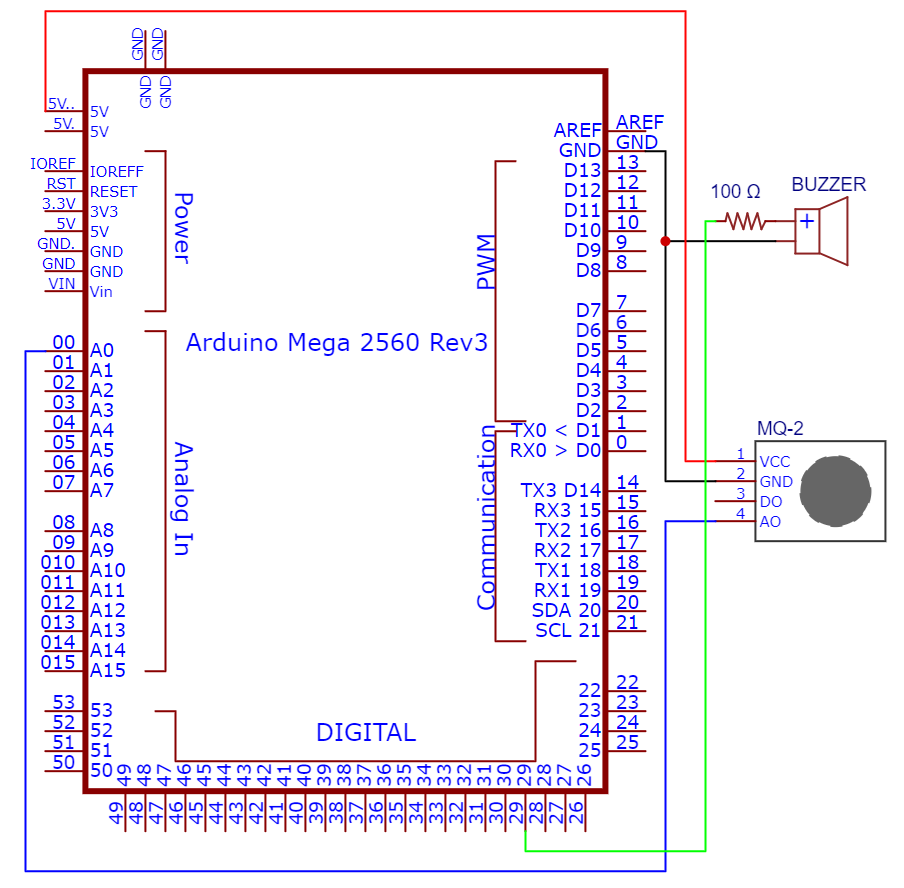
\includegraphics[width=0.7\textwidth, height=0.7 \textwidth]{bachelors_ro/images/conexiune_mq2_buzzer.png}
\caption{Schema de conectare a senzorului de gaz și fum și al buzzer-ului}
\label{fig:conexiune_mq2_buzzer}
\end{figure}

\section{Conectarea Senzorului PIR și al led-ului aferent si al modulului cu fotorezistor și al led-ului aferent}
Primul ansamblu are ca scop aprinderea led-ului în momentul în care senzorul PIR detectează mișcare. Pentru a fi conectat la placa de dezvoltare, led-ul are nevoie de o rezistență de 220 Ohm pe firul de alimentare ce este legat la un pin digital (D26). Rezistența este folistă pentru a limita curentul ce trece prin led pentru a evita arderea acestuia, valoarea este calculată folosind legea lui Ohm ($I=U/R$). Celălalt picior al led-ului este legat la pinul GND. Senzorul PIR dispune de 3 pini: VCC, Dout, GND. Pinul VCC este legat la pinul 5 V de pe placă, pinul de GND la pinul GND al plăcii, iar Dout la pinul digital D4.

Cel de-al doilea ansamblu are ca scop aprinderea led-ului în funcție de nivel de lumină detectat de modulul cu fotorezistor. Led-ul aferent modului este legat în același fel ca și la ansamblul anterior cu mențiunea ca acesta este conectat la pinul D24. Modulul cu fotorezistor dispune de aceeași 3 pini ca și senzorul PIR. Modulul de legătură este similar cu excepția faptului că pinul Dout al modulului este legat la pinul digital D8 al plăcii Arduino.

În figura \ref{fig:conexiune_pir_lum_led} este prezentat montajul final pentru senzorul PIR, modulul cu fotorezistor și led-uri.

\begin{figure}[H]
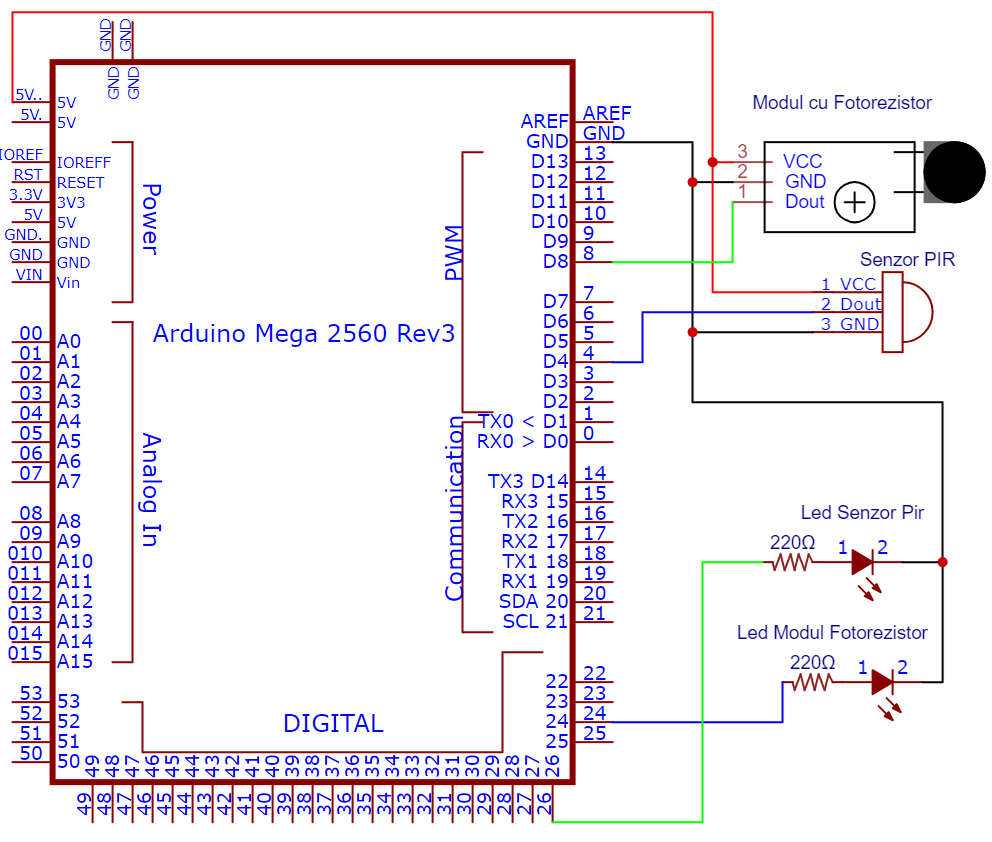
\includegraphics[width=0.8\linewidth]{bachelors_ro/images/conexiune_pir_lum_led.png}
\caption{Schema de conectare a senzorului PIR, a modulului cu fotorezistor și a led-urilor aferent}
\label{fig:conexiune_pir_lum_led}
\end{figure}